\section{Surrogate Models}
%-----------------------------------------------------------------------
\begin{frame}[c]{Surrogate Models}
\framesubtitle{Desiderata}

\begin{columns}[T] % align columns
\begin{column}{.48\textwidth}
\only<1-2>{
    \begin{block}{Mandatory}
    \begin{itemize}
    	\item Regression model
    	\item Uncertainty estimates
    	\item Accurate predictions
    \end{itemize}
    \end{block}
}
\only<2-2>{
    \begin{block}{Depending on the application}
    \begin{itemize}
    	\item Cheap-to-train
    	\item Scales with the complexity of the data
    	\note[item]{(number of features and observations)}
    	\item Can handle different types of inputs
    	\note[item]{(categorical and continuous)}
    \end{itemize}
    \end{block}
}
\end{column}%

\hfill%

\begin{column}{.48\textwidth}

%\only<1-1>{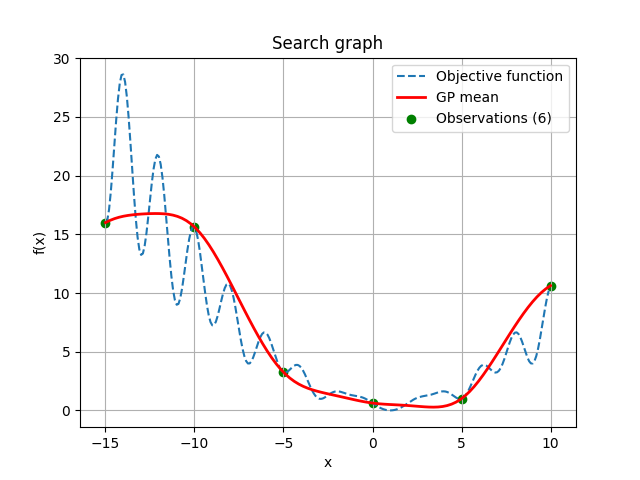
\includegraphics[width=1.\textwidth]{images/bo_loop_overview/03_mean.png}}
%\only<2-6>{
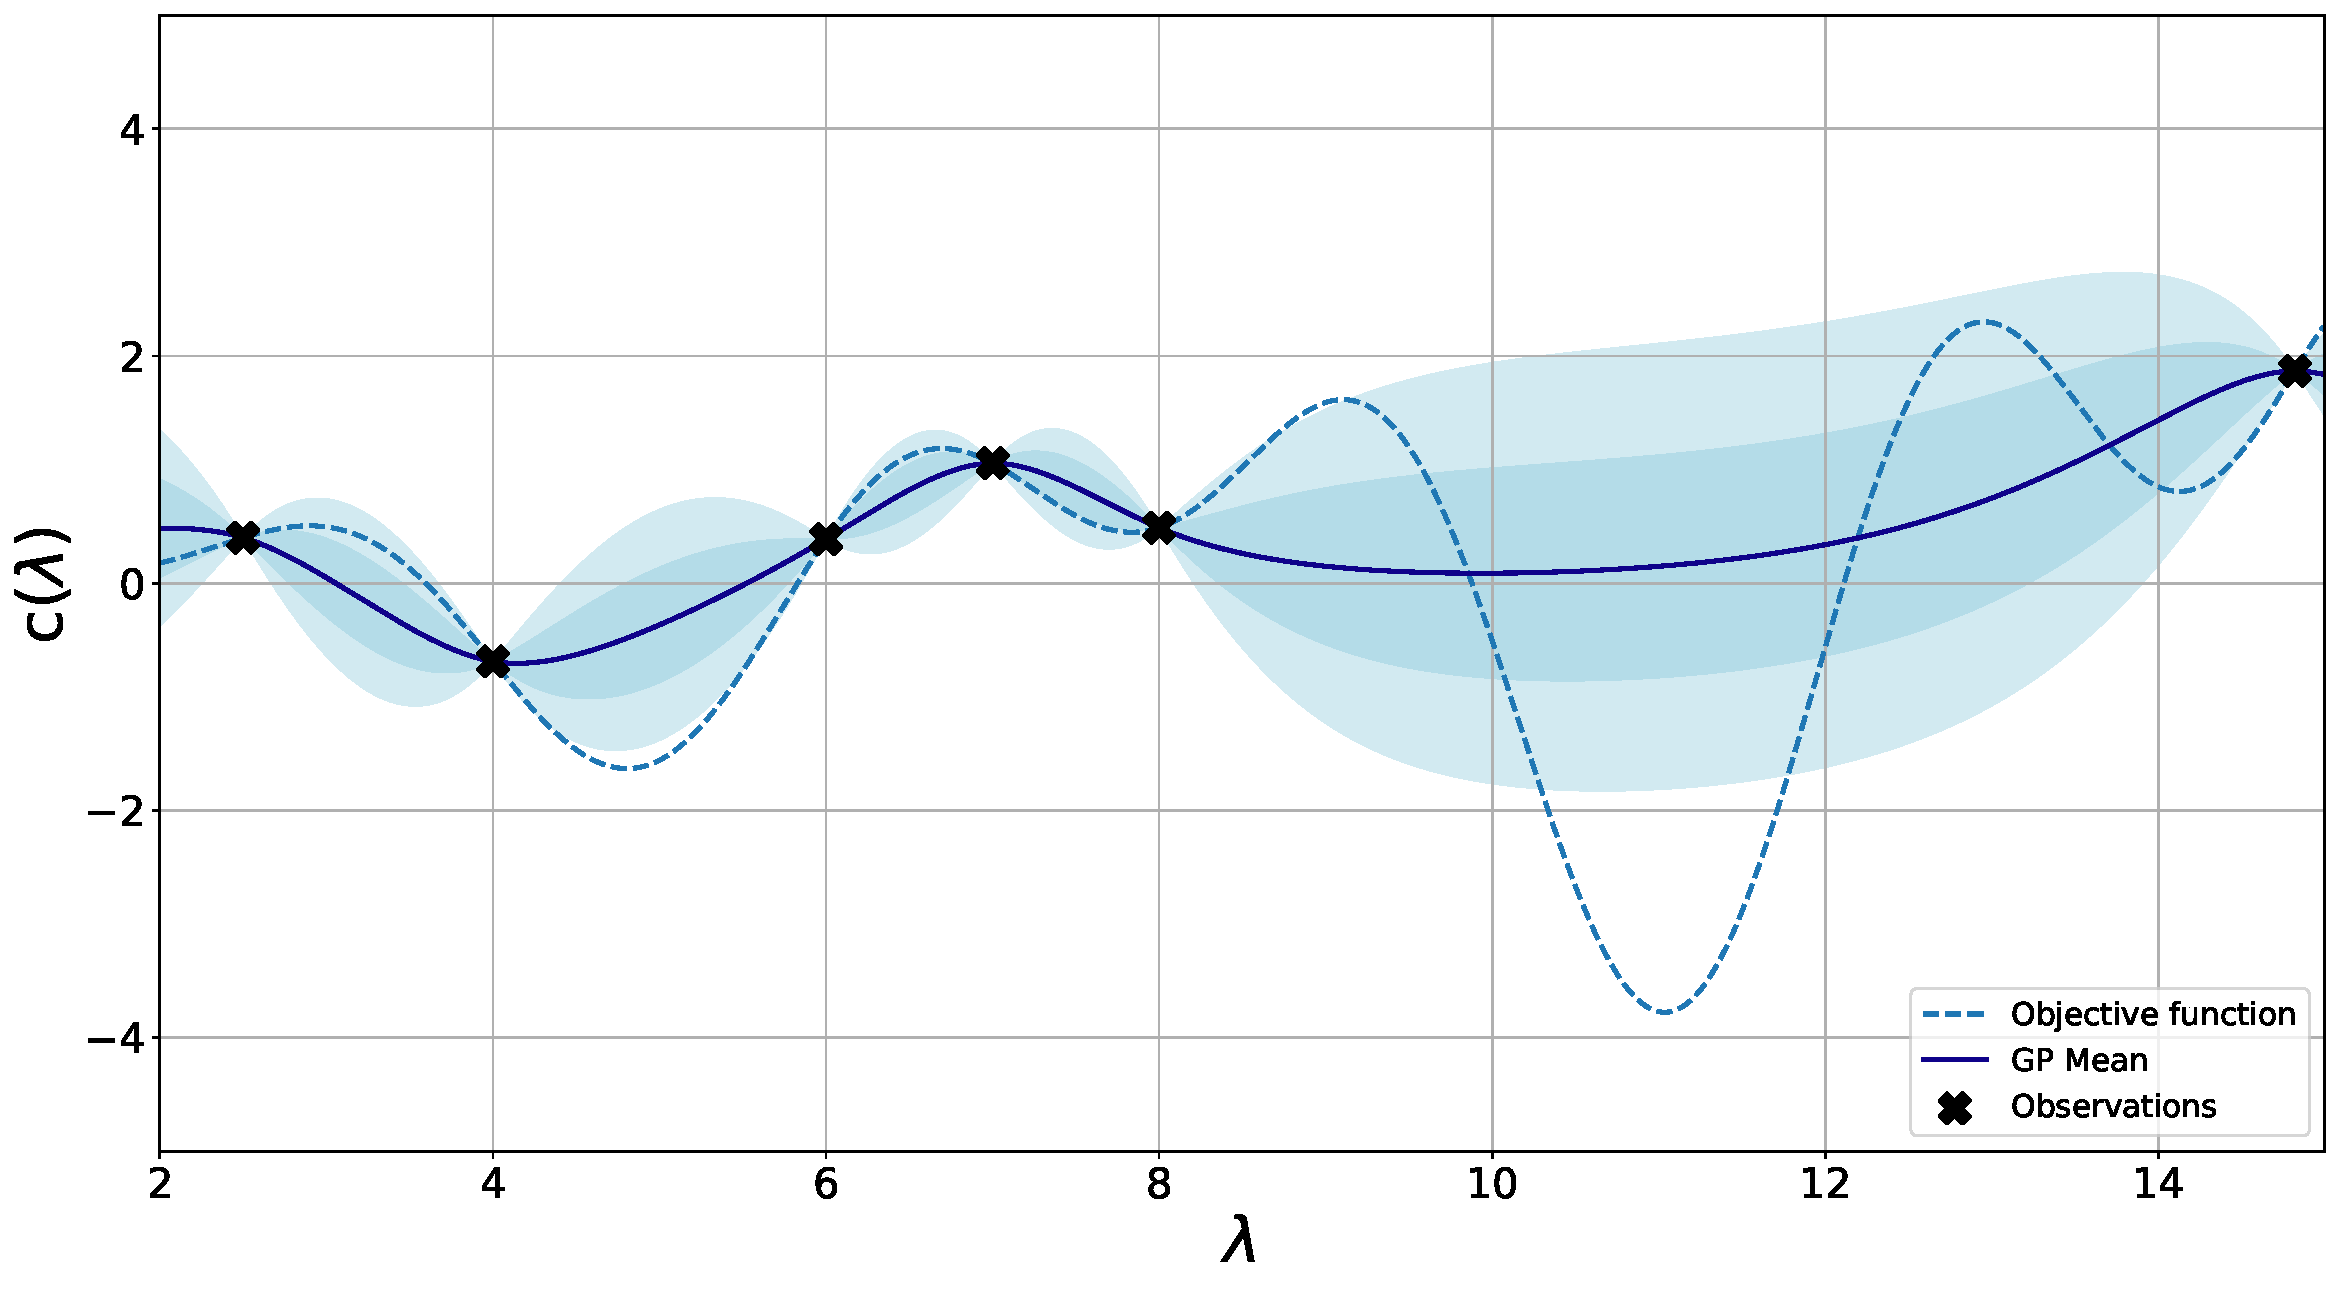
\includegraphics[width=\textwidth]{w06_hpo_bo/images/bo_loop_overview/Uncertainty.pdf}
%}

\end{column}%
\end{columns}

\end{frame}
%-----------------------------------------------------------------------

%-----------------------------------------------------------------------
%-----------------------------------------------------------------------
\begin{frame}[c]{Surrogate Models}
\framesubtitle{Overview}

\begin{columns}[T] % align columns
\begin{column}{.38\textwidth}
\begin{minipage}[c][.6\textheight][c]{\linewidth}
\begin{itemize}
	\item Gaussian Processes \note[item]{(quite common)}
	\item Random Forests \note[item]{(our default choice)}
	\item Bayesian Neural Networks \note[item]{(recent trend)}

\end{itemize}
\end{minipage}
\end{column}%

\hfill%

\begin{column}{.58\textwidth}

\begin{columns}[T] % align columns
\begin{column}{.48\textwidth}
    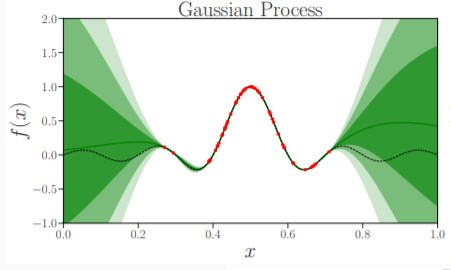
\includegraphics[width=1.\textwidth]{images/surrogate_models/uncertainty_gp.jpg}
\end{column}%

\hfill%

\begin{column}{.48\textwidth}
    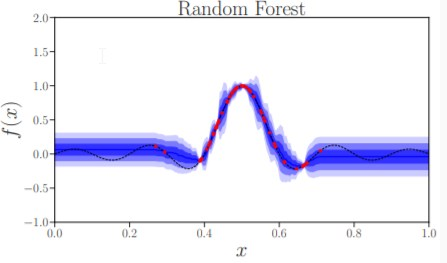
\includegraphics[width=1.\textwidth]{images/surrogate_models/uncertainty_forest.jpg}
\end{column}%
\end{columns}

\vspace*{\fill}
\begin{center}
  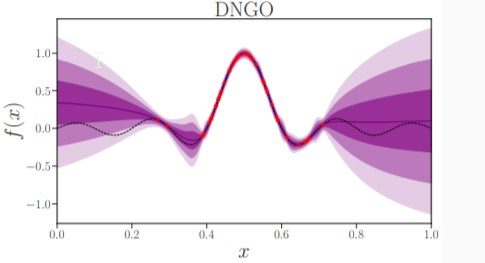
\includegraphics[width=.6\textwidth]{images/surrogate_models/uncertainty_dngo.jpg}
\end{center}
\vspace*{\fill}

\end{column}%
\end{columns}

\source{A. Klein: Introduction Automated Machine Learning}

%% TODO
\comment{adjust those plots
FH: best to have plots stay on the slide, e.g., next to each other.}

\end{frame}
%-----------------------------------------------------------------------
\begin{frame}[c]{Surrogate Models}
\framesubtitle{Gaussian Processes - Reminder}

\begin{columns}[T] % align columns
\begin{column}{.48\textwidth}

    \begin{block}{Advantages}
    \begin{itemize}
    	\item Smooth and reliable uncertainty estimates 
		\item Sample efficiency
    	\item We can encode expert knowledge about the design space in the kernel 
    \end{itemize}
    \end{block}
\end{column}%

\hfill%
\pause

\begin{column}{.48\textwidth}
    \begin{block}{Disadvantages}
    \begin{itemize}
    	\item We have to define a good kernel for each application 
    	\note[item]{(if we don't optimize small-dimensional, continuous functions)}
    	\item Cost scales cubically with the number of observations 
    	\note[item]{(because of inverting the kernel)}
    	\item Not easily applicable in discrete or conditional spaces 
    	\item Sensitive to its own hyperparameters
    \end{itemize}
\end{block}

\end{column}
\end{columns}

\note[item]{
	\begin{itemize}
		 \item e.g., special kernels for categorical hyperparameters and\\ conditional dependencies
	\end{itemize}
}
	
\note[item]{
    \begin{itemize}
    	\item to address this issue, there are sparse GPs\\ \lit{Snelson and Ghahramani. 2005}
    \end{itemize}
}

\end{frame}
%-----------------------------------------------------------------------

%-----------------------------------------------------------------------
%-----------------------------------------------------------------------
%\begin{frame}[c]{Gaussian Processes - reminder}
%
%\begin{itemize}
%    \item<1-3> The prior is a GP with constant mean and variance; draws are jointly Gaussian
%    \item<2-3> The kernel (covariance) function $K$ tells us how correlated the function values at two points are
%    \item<3-3> The posterior is also a GP, with predictive distribution:
 %   \begin{equation*}
 %        P(\func_{\bocount+1} \vert \dataset_{1:\bocount}, \conf_{\bocount+1}) =  \mathcal{N}(\mean_{\bocount}(\conf_{\bocount+1}), \variance_{\bocount}(\conf_{\bocount+1}))
 %   \end{equation*}
 %   \begin{equation*}
 %       \mean_{\bocount}(\conf_{\bocount+1}) = \bm{k}^{T} \bm{K}^{-1} \bm{\func_{1:\bocount}}
 %   \end{equation*}
 %   \begin{equation*}
 %       \variance_{\bocount}(\conf_{\bocount+1}) = k(\conf_{\bocount+1}, \conf_{\bocount+1}) - \bm{k}^{T} \bm{K}^{-1} \bm{k}
 %   \end{equation*}
%\end{itemize}
%
%\note[item]{for the review of GPs - Rasmussen and Williams}
%
%\end{frame}
%-----------------------------------------------------------------------
 
% %-----------------------------------------------------------------------
% %-----------------------------------------------------------------------
% \begin{frame}[c]{Surrogate Models: GPs - kernel hyperparameters}

% \begin{itemize}
%     \item After choosing the kernel, we must also manage the hyperparameters that govern its behaviour, as well as that of the mean function.  \pause
%     \item For our problems of interest, typically we have $D + 3$ GPs hyperparameters:  
%     \begin{itemize}
%         \item $D$ length scales $\theta_{1:D}$, 
%         \item the covariance amplitude $\theta_{0}$, 
%         \item the observation noise $\noise$, 
%         \item a constant mean $\mean$. 
%     \end{itemize}
% \end{itemize}

% \end{frame}
% %-----------------------------------------------------------------------


%-----------------------------------------------------------------------
%-----------------------------------------------------------------------
\begin{frame}[c]{Surrogate Models}
\framesubtitle{Gaussian Processes - Kernel Hyperparameters}

\begin{itemize}
    \item We can use \emph{Maximum A Posteriori} (MAP) or \emph{Maximum Likelihood Estimation} (MLE) to optimize hyperparameters of the Gaussian process.
    \item However, it is not realistic to assume that the hyperparameters distribution can be represented by a single point estimate
\end{itemize}

\end{frame}
%-----------------------------------------------------------------------
\begin{frame}[c]{Surrogate Models}
\framesubtitle{Gaussian Processes - Kernel Hyperparameters}

\begin{columns}[T] % align columns
\begin{column}{.6\textwidth}
\begin{itemize}
    \item<+-> \emph{Markov-Chain Monte-Carlo} (MCMC) samples hyperparameters from the posterior distribution
    \item<+-> \emph{Marginalize} over hyperparameters and compute an \emph{integrated acquisition function}:
        \begin{equation*}
        \begin{aligned}
            \Bar{\acq}(\conf) = \int \acq (\conf, \surro_\theta)p(\theta)d\theta
        \end{aligned}
        \end{equation*}
    \item<+-> But, MCMC is computationally more expensive since the acquisition function now needs to be calculated more than once.
\end{itemize}
\end{column}
%
\begin{column}{.4\textwidth}
\only<2->{
\begin{figure}
    \centering
    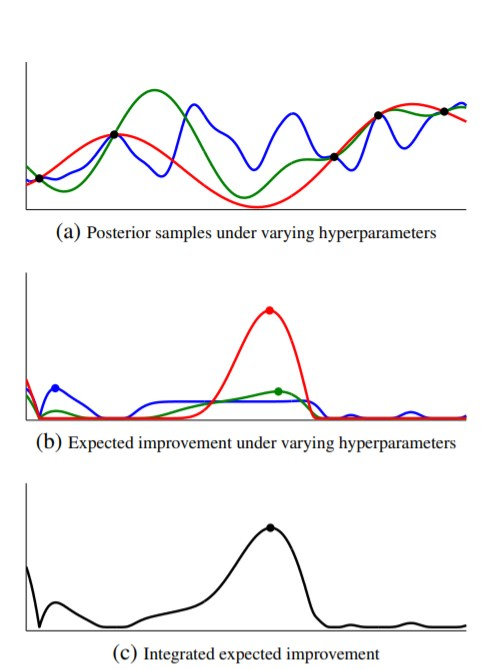
\includegraphics[width=0.7\textwidth]{images/surrogate_models/kernel_hp_mcmc.jpg}
\end{figure}}
\end{column}

\end{columns}

\source{Snoek et al. 2015}
\end{frame}
%-----------------------------------------------------------------------
\begin{frame}[c]{Surrogate Models}
\framesubtitle{Random Forests}

\centering
    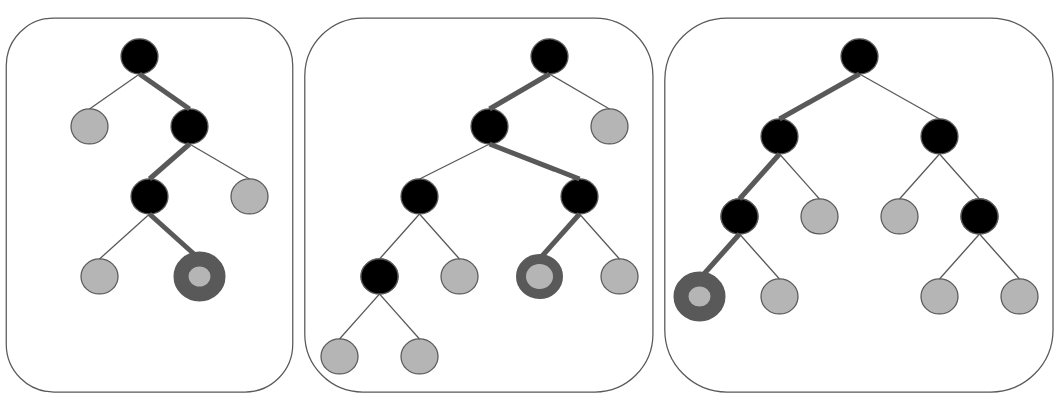
\includegraphics[width=0.5\textwidth]{images/surrogate_models/random_forest_pic}

\begin{columns}[T] % align columns
\begin{column}{.48\textwidth}

\begin{block}{Train}
\begin{itemize}
	\item $n$ randomized regression trees
	\item Subsampled training data for each tree (with bootstrapping)
	\item Each tree gives us a possible explanation for the observations
\end{itemize}
\end{block}
\end{column}

\pause
\hfill

\begin{column}{.48\textwidth}
    \begin{block}{Predict}
    \begin{itemize}
    	\item Obtain prediction of each tree
    	\item Aggregate predictions (e.g., average)
    	\item Uncertainty of predictions: stdev across tree predictions
    \end{itemize}
    \end{block}
\end{column}
\end{columns}

\end{frame}
%-----------------------------------------------------------------------
\begin{frame}[c]{Surrogate Models}
\framesubtitle{Random Forests - Hyperparameters}

\begin{columns}
	\column{0.5\textwidth}
	\centering
	w bootstrapping and\\ w/o random splits
	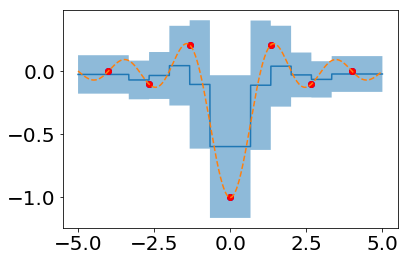
\includegraphics[width=0.5\textwidth]{images/surrogate_models/rf_boot_middle_split.png}

	w bootstrapping and\\ w/ random splits
	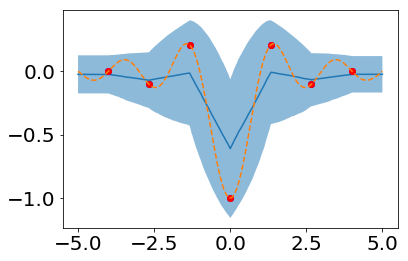
\includegraphics[width=0.5\textwidth]{images/surrogate_models/rf_boot_rand_split.png}

	\column{0.5\textwidth}
	\centering
	w/o bootstrapping and\\ w/o random splits
	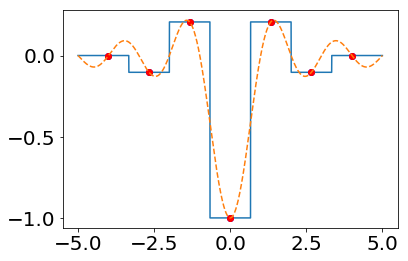
\includegraphics[width=0.5\textwidth]{images/surrogate_models/rf_noboot_middle_split.png}
	
	w/o bootstrapping and\\ w/ random splits
	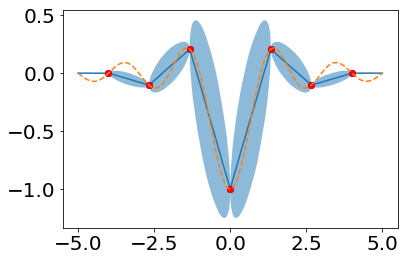
\includegraphics[width=0.5\textwidth]{images/surrogate_models/rf_noboot_rand_split.png}
\end{columns}

\end{frame}
%-----------------------------------------------------------------------
\begin{frame}[c]{Surrogate Models}
\framesubtitle{Random Forests - Summary}

\begin{columns}[T] % align columns
\begin{column}{.48\textwidth}

    \begin{block}{Advantages}
    \begin{itemize}
        \item Cheap to train 
        \item Scales well with \#observations: 
        \begin{itemize}
        	\item Worst-case complexity for $T$ tress with $n$ data points of dimensionality $p$: $\mathcal O(T\cdot p \cdot n^2 \log{n})$. 
        \end{itemize}
        \item Training can be parallelized 
        \item Can easily handle conditional, categorical, continuous and discrete spaces 
        \item Quite robust against its own hyperparameters
    \end{itemize}
    \end{block}
\end{column}%

\hfill%
\pause

\begin{column}{.48\textwidth}
    \begin{block}{Disadvantages}
    \begin{itemize}
        \item Poor uncertainty estimates 
        \item Poor extrapolation (constant) 
    	\item Priors cannot be incorporated easily 
    \end{itemize}
    \end{block}

\end{column}
\end{columns}

\end{frame}
%-----------------------------------------------------------------------
\begin{frame}[c]{Surrogate Models}
\framesubtitle{Bayesian Neural Networks}

\begin{itemize}
    \item Extend regression NNs to model uncertainty
    \item Deal with all sources of parameter uncertainty: \pause
    \begin{itemize}
        \item More than one weight vector can explain the observed data 
        \item Take into account all possible explanations 
    \end{itemize}

\centering
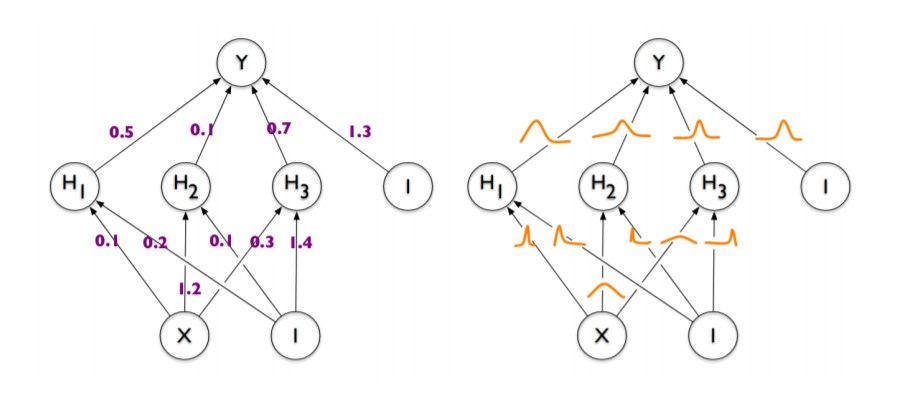
\includegraphics[width=0.6\textwidth]{images/surrogate_models/bnn.jpg}

\end{itemize}

\source{\href{http://proceedings.mlr.press/v37/blundell15.pdf}{Blundell et al. 2015}}

\end{frame}
%-----------------------------------------------------------------------
%\begin{frame}[c]{Surrogate Models: Bayesian Neural Networks - Idea}
%
%\begin{itemize}
%    \item Extend regression NNs to model uncertainty
%    \item Deal with all sources of parameter uncertainty
%    \item If possible, one would also deal with uncertainty about the network architecture
%     \begin{itemize}
%        \item For every architecture, one would still want to be Bayesian about its weights... 
%        \item Nobody is really Bayesian about architectures these days 
%        \item This has been too expensive; but that may change with efficient gradient-based architecture search methods...
%    \end{itemize}
%\end{itemize}
%
%\end{frame}
%-----------------------------------------------------------------------

\begin{frame}[c]{Surrogate Models}
\framesubtitle{Bayesian Neural Networks - Approaches}

\begin{itemize}
	\item Standard Bayesian optimization model Gaussian process scales badly to a large number of data points
	\item Bayesian Neural Networks can be used as a more scalable model\pause
	\bigskip
	\item Overview of Bayesian Neural Networks for BO:
	\begin{itemize}
	    \item \lit{\href{https://arxiv.org/pdf/1502.05700.pdf}{Snoek et al. 2015}} Scalable Bayesian Optimization Using Deep Neural Networks
	    \item \lit{\href{https://www.ismll.uni-hildesheim.de/pub/pdfs/schilling2015-ecml.pdf}{Schilling et al. 2015}} Hyperparameter Optimization with Factorized Multilayer Perceptrons
	    \item \lit{\href{https://papers.nips.cc/paper/6117-bayesian-optimization-with-robust-bayesian-neural-networks.pdf}{Springenberg et al. 2016}} Bayesian Optimization with Robust Bayesian Neural Networks
	    \item \lit{\href{https://arxiv.org/abs/1706.01825}{Hern\'andez-Lobato et al. 2017}} Parallel and Distributed Thompson Sampling for Large-scale Accelerated Exploration of Chemical Space
        \item \lit{\href{https://papers.nips.cc/paper/7917-scalable-hyperparameter-transfer-learning}{Perrone et al. 2018}} Scalable Hyperparameter Transfer Learning

	\end{itemize}
\end{itemize}

\end{frame}
%-----------------------------------------------------------------------

\begin{frame}[c]{Surrogate Models}
\framesubtitle{Bayesian Neural Networks - DNGO}

First approach: \href{https://arxiv.org/pdf/1502.05700.pdf}{Scalable Bayesian Optimization Using Deep Neural Networks}

\begin{itemize}
    \item Fit a standard neural network to the data 
    \item Use the representation in the last hidden layer as basis \\ functions $\phi(x)$ of the input $x$ 
    \item Use Bayesian linear regression for the output layer \pause
    \begin{itemize}
        \item The last layer is linear in its parameters $\theta$  
        \item Therefore, the Bayesian linear regression formulas work directly 
        \item Feasible in closed form, in time $O(N d^3)$, \\ where $N$ is the number of data points and $d$ is the number of \\ hidden units in the last layer 
    \end{itemize}
    \item Not fully Bayesian yet
\end{itemize}

\vspace{1cm}
\hspace{12cm}
\lit{\href{https://arxiv.org/pdf/1502.05700.pdf}{Snoek et al. 2015}}

\end{frame}
%-----------------------------------------------------------------------
\begin{frame}[c]{Surrogate Models}
\framesubtitle{Bayesian Neural Networks}

\begin{columns}[T] % align columns
\begin{column}{.48\textwidth}

    \begin{block}{Advantages}
    \begin{itemize}
        \item Scales linearly with \#observations 
        \item Given enough network samples obtain nice and smooth uncertainty estimates 
        \item Can handle categorical, continuous and discrete spaces
    \end{itemize}
    \end{block}
\end{column}%

\hfill%
\pause

\begin{column}{.48\textwidth}
    \begin{block}{Disadvantages}
    \begin{itemize}
        \item Poorer uncertainty estimates 
        \item Many meta-design decisions 
    	\item No robust off-the-shelf implementation 
    	\item Usually needs more data than Gaussian processes
    \end{itemize}
    \end{block}

\end{column}
\end{columns}

\end{frame}
%-----------------------------------------------------------------------
\begin{frame}[c]{Surrogate Models}
\framesubtitle{Bayesian Neural Networks - Further Reading}

There's a lot more which hasn't been applied to Bayesian optimization yet
\begin{itemize}
        \item \lit{\href{https://www.cs.utoronto.ca/~radford/bnn.book.html}{Neal 1995}} Bayesian Learning for Neural Networks
        \item \lit{\href{https://www.microsoft.com/en-us/research/uploads/prod/2006/01/Bishop-Pattern-Recognition-and-Machine-Learning-2006.pdf}{Bishop 2006}} Pattern Recognition and Machine Learning
        \item \lit{\href{https://papers.nips.cc/paper/7219-simple-and-scalable-predictive-uncertainty-estimation-using-deep-ensembles.pdf}{Lakshminarayanan et al. 2017}}: Simple and Scalable Predictive Uncertainty Estimation using Deep Ensembles
        \item \lit{\href{https://arxiv.org/abs/1506.02142}{Gal et al. 2016}} Dropout as a Bayesian Approximation:
        Representing Model Uncertainty in Deep Learning
        \item \lit{\href{https://arxiv.org/abs/1802.06455}{Teye et al. 2018}} Bayesian Uncertainty Estimation for Batch Normalized Deep Networks
        \item \lit{\href{https://arxiv.org/abs/1704.00109}{Gao Huang et al. 2017}} Snapshot Ensembles: Train 1, get M for free
\end{itemize}
or maybe doesn't work and hasn't been published
\end{frame}
%-----------------------------------------------------------------------
\begin{frame}[c]{Questions to Answer for Yourself / Discuss with Friends}

\begin{itemize}
    %GP
    \item \emph{Repetition.} What are the most important hyperparameters of a GP that you would want to optimize for Bayesian Optimization? 
    %RF
    \item \emph{Discussion.} For which optimization problems would you rather use a RF than a GP?
    %BNN
    \item \emph{Discussion.} Can a BNN be trained with standard MCMC in theory and in practice?
    %DNGO
    \item \emph{Discussion.} Why can't you use a Bayesian Linear Regression for all layers in a Deep Neural Network?
\end{itemize}
\end{frame}
